%
% File acl2018.tex

\documentclass[11pt,a4paper]{article}
\usepackage[hyperref]{acl2019}
\usepackage[T1]{fontenc}
\usepackage{times}
\usepackage{latexsym}
\usepackage{amsmath}
\usepackage{tikz}
\usepackage{tikz-dependency}
\usepackage[warn]{textcomp}
\usepackage[font=small]{caption}
\usepackage{subcaption}
\usepackage{multirow}
\usepackage{url}
\usepackage{etoolbox}
\usepackage{xr}

\hyphenation{SemEval}


\usetikzlibrary{shapes,shapes.misc}

%\aclfinalcopy % Uncomment this line for the final submission

%\setlength\titlebox{5cm}
% You can expand the titlebox if you need extra space
% to show all the authors. Please do not make the titlebox
% smaller than 5cm (the original size); we will check this
% in the camera-ready version and ask you to change it back.

\title{Multitask Parsing Across Semantic Representations}

\author{Daniel Hershcovich$^{1,2}$ \\
  \\\And
  Omri Abend$^2$ \\
  $^1$The Edmond and Lily Safra Center for Brain Sciences \\
  $^2$School of Computer Science and Engineering \\
  Hebrew University of Jerusalem \\
  \texttt{\{danielh,oabend,arir\}@cs.huji.ac.il}
  \\\And
  Ari Rappoport$^2$
}

\date{}

\begin{document}

\maketitle

  We
  tackle the challenging task of improving semantic parsing
  performance, by multitask learning with UCCA \cite{abend2013universal},
  AMR \cite{banarescu2013abstract}, SDP \cite{oepen2016towards} and UD \cite{nivre2016universal} parsing.
While these schemes are formally different and focus on different distinctions,
much of their semantic content is shared \cite{abend2017state}.
  We experiment on three languages,
  using a uniform transition-based system and learning 
  architecture.


%%%%%%%%%%%%%%%%%%%%%%%%%%%%%%%%%%%%%%%%%%%%%%%%%%%%%%%%%%%%%%%%%%%%%%%%%%%%%%%%%%%%%%%%
\section*{General Transition-based DAG Parser}\label{sec:model}
We extend TUPA \cite{hershcovich2017a}, 
a transition-based parser 
originally developed for UCCA.
TUPA's transition system can yield any labeled DAG
whose terminals are anchored in the text tokens.
To support parsing into AMR, which uses graphs that are not anchored in the tokens,
 we take advantage of existing alignments of the graphs with the text
tokens during training.


To apply our parser to the four target tasks,
we convert them into a unified DAG format, which is inclusive enough to
allow representing any of the schemes with very little loss of information.

\begin{figure}[!ht]
\begin{subfigure}{0.23\textwidth}
    \centering
    \scalebox{.5}{
    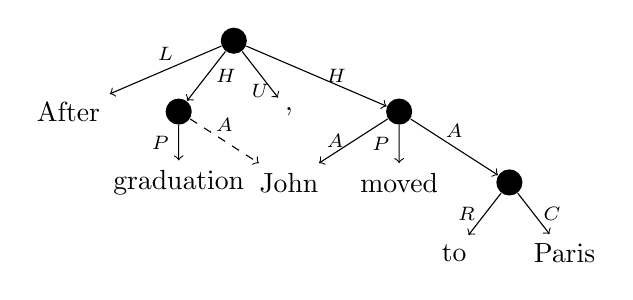
\begin{tikzpicture}[level distance=9mm, sibling distance=14mm, ->,
        every circle node/.append style={fill=black}]
      \tikzstyle{word} = [font=\rmfamily,color=black]
      \node (ROOT) [circle] {}
        child {node (After) [word] {After} edge from parent node[above] {\scriptsize $L$}}
        child {node (graduation) [circle] {}
        {
          child {node [word] {graduation} edge from parent node[left] {\scriptsize $P$}}
        } edge from parent node[right] {\scriptsize $H$} }
        child {node [word] {,} edge from parent node[below] {\scriptsize $U$}}
        child {node (moved) [circle] {}
        {
          child {node (John) [word] {John} edge from parent node[left] {\scriptsize $A$}}
          child {node [word] {moved} edge from parent node[left] {\scriptsize $P$}}
          child {node [circle] {}
          {
            child {node [word] {to} edge from parent node[left] {\scriptsize $R$}}
            child {node [word] {Paris} edge from parent node[right] {\scriptsize $C$}}
          } edge from parent node[above] {\scriptsize $A$} }
        } edge from parent node[right] {\scriptsize $H$} }
        ;
      \draw[dashed,->] (graduation) to node [above] {\scriptsize $A$} (John);
    \end{tikzpicture}}
  \caption{UCCA}
  \label{fig:converted_example_ucca}
\end{subfigure}
\begin{subfigure}{0.23\textwidth}
  \centering
  \scalebox{.5}{
  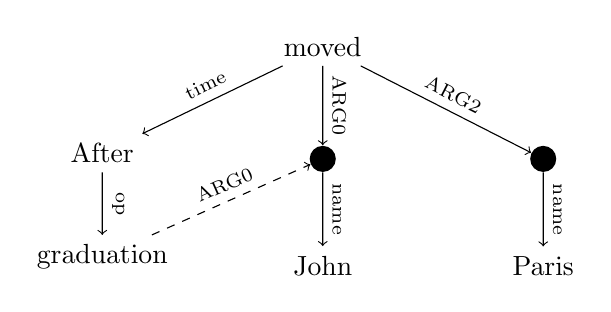
\begin{tikzpicture}[level distance=16mm, ->,
      every node/.append style={sloped,anchor=south,auto=false,font=\scriptsize},
      level 1/.style={sibling distance=28mm},
      level 2/.style={sibling distance=14mm},
      level 3/.style={sibling distance=12mm}]
    \tikzstyle{word} = [font=\rmfamily,color=black]
    \node (ROOT) [word] {moved}
      child {node [word] {After}
      {
            child {node (graduation) [word] {graduation} edge from parent node {op} }
      } edge from parent node {time} }
      child {node (John) [fill=black,circle] {}
      {
        child {node [word] {John} edge from parent node {name} }
      } edge from parent node {ARG0} }
      child {node [fill=black,circle] {}
      {
        child {node [word] {Paris} edge from parent node {name} }
      } edge from parent node {ARG2} }
      ;
      \draw[dashed] (graduation) to node {ARG0} (John);
  \end{tikzpicture}}
  \captionof{figure}{AMR}
  \label{fig:converted_example_amr}
\end{subfigure}
\begin{subfigure}{0.23\textwidth}
  \centering
  \scalebox{.5}{
  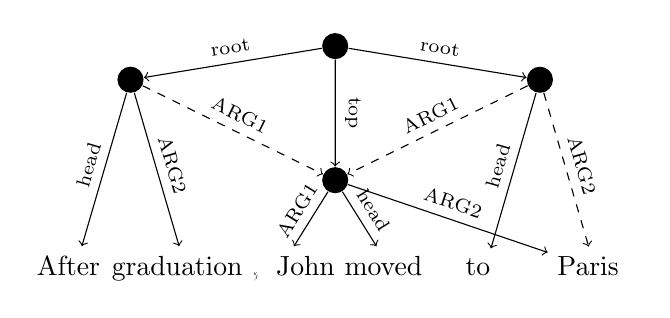
\begin{tikzpicture}[level distance=12mm, ->,
      every node/.append style={sloped,anchor=south,auto=false,font=\scriptsize},
      level 1/.style={sibling distance=26mm,level distance=6mm},
      level 2/.style={sibling distance=14mm,level distance=14mm}]
    \tikzstyle{word} = [font=\rmfamily,color=black]
    \node (ROOT) [fill=black,circle] {}
      child {node (after) [fill=black,circle] {}
      {
        child {node [draw=none] {}
        {
          child {node [word] (after_word) {After{\color{white}g}} edge from parent [draw=none]}
        } edge from parent [draw=none] }
        child {node [draw=none] {}
        {
          child {node [word] (graduation) {graduation ,} edge from parent [draw=none]}
        } edge from parent [draw=none] }
      } edge from parent node {root}}
      child {node [draw=none] {}
      {
        child {node (moved) [fill=black,circle] {}
        {
          child {node [word] {\quad{\color{white}g} John} edge from parent node {ARG1}}
          child {node [word] {moved{\color{white}g}} edge from parent node {head}}
        } edge from parent [draw=none] }
      } edge from parent [draw=none] }
      child {node (to) [fill=black,circle] {}
      {
        child {node [draw=none] {}
        {
            child {node [word] (to_word) {to{\color{white}g}} edge from parent [draw=none]}
          } edge from parent [draw=none] }
          child {node [draw=none] {}
        {
          child {node [word] (Paris) {Paris{\color{white}g}} edge from parent [draw=none]}
        } edge from parent [draw=none] }
      } edge from parent node {root}}
      ;
      \draw (ROOT) to node {top} (moved);
      \draw (after) to node {head} (after_word);
      \draw (after) to node {ARG2} (graduation);
      \draw[dashed] (after) to node {ARG1} (moved);
      \draw[dashed] (to) to node {ARG1} (moved);
      \draw (to) to node {head} (to_word);
      \draw (moved) to node {ARG2} (Paris);
      \draw[dashed] (to) to node {ARG2} (Paris);
  \end{tikzpicture}}
  \captionof{figure}{DM}
  \label{fig:converted_example_sdp}
\end{subfigure}
\begin{subfigure}{0.23\textwidth}
  \centering
  \scalebox{.5}{
  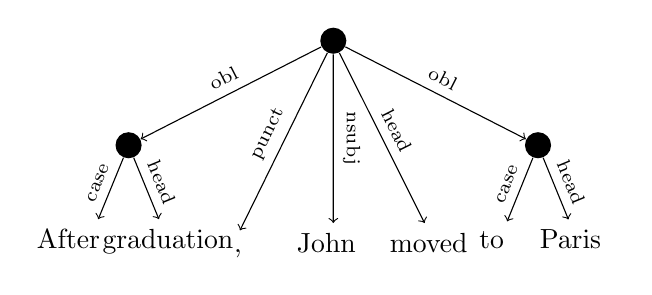
\begin{tikzpicture}[level distance=15mm, ->,
      every node/.append style={sloped,anchor=south,auto=false,font=\scriptsize},
      level 1/.style={sibling distance=13mm},
      level 2/.style={sibling distance=1cm}]
    \tikzstyle{word} = [font=\rmfamily,color=black]
    \node (ROOT) [fill=black,circle] {}
      child {node (after) [fill=black,circle] {}
      {
        child {node [word] {After{\color{white}g}\quad\quad} edge from parent node {case}}
        child {node [word] {\quad graduation\quad\quad} edge from parent node {head}}
      } edge from parent node {obl}}
      child {node {}
      {
        child {node [word] (comma) {\quad,{\color{white}g}} edge from parent [draw=none]}
      } edge from parent [draw=none]}
      child {node {}
      {
        child {node [word] (John) {John{\color{white}g}} edge from parent [draw=none]}
      } edge from parent [draw=none]}
      child {node {}
      {
        child {node [word] (moved) {moved{\color{white}g}} edge from parent [draw=none]}
      } edge from parent [draw=none]}
      child {node (to) [fill=black,circle] {}
      {
          child {node [word] {to{\color{white}g}} edge from parent node {case}}
          child {node [word] {Paris{\color{white}g}} edge from parent node {head}}
      } edge from parent node {obl}}
      ;
      \draw (ROOT) to node {punct} (comma);
      \draw (ROOT) to node {nsubj} (John);
      \draw (ROOT) to node {head} (moved);
  \end{tikzpicture}}
  \captionof{figure}{UD}\label{fig:converted_example_ud}
\end{subfigure}

\caption*{Graphs after conversion to unified DAG format.}\label{fig:converted_examples}
\end{figure}


%%%%%%%%%%%%%%%%%%%%%%%%%%%%%%%%%%%%%%%%%%%%%%%%%%%%%%%%%%%%%%%%%%%%%%%%%%%%%%%%%%%%%%%%%%%%
\section*{Multitask Transition-based Parsing}\label{sec:multitask}

As the same model can be applied to different tasks, 
we train it in a multitask setting.
The fairly small training set available for UCCA
makes MTL particularly appealing,
and we focus on it, treating AMR, DM and UD parsing as auxiliary tasks.

Improvements from using MTL are substantial in English, German and French.
The best MTL models are significantly better than single-task models,
demonstrating that even a small training set for the main task may suffice,
given enough auxiliary training data.

  Despite notable conceptual, formal and domain differences,
  we show that multitask learning significantly improves UCCA parsing
  in both in-domain and out-of-domain settings.


\begin{table}[h]
\centering
\small
\setlength\tabcolsep{3pt}
\begin{tabular}{l|lll|lll}
& \multicolumn{3}{c|}{\footnotesize \bf Primary} & \multicolumn{3}{c}{\footnotesize \bf Remote} \\
& \footnotesize \textbf{LP} & \footnotesize \textbf{LR} & \footnotesize \textbf{LF}
& \footnotesize \textbf{LP} & \footnotesize \textbf{LR} & \footnotesize \textbf{LF} \\
\hline
\multicolumn{4}{l|}{\small \bf English (in-domain)} & \\
\footnotesize Single
& 74.4 & 72.9 & 73.6 & 53 & 50 & 51.5 \\
\cline{1-1}
\footnotesize AMR
& 74.7 & 72.8 & 73.7 & 48.7$\star$ & 51.1 & 49.9 \\
\footnotesize DM
& 75.7$\star$ & 73.9$\star$ & 74.8$\star$ & 54.9 & 53 & \textbf{53.9} \\
\footnotesize UD
& 75$\star$ & 73.2 & 74.1$\star$ & 49 & 52.7 & 50.8 \\
\footnotesize AMR + DM
& 75.6$\star$ & 73.9$\star$ & 74.7$\star$ & 49.9 & 53 & 51.4 \\
\footnotesize AMR + UD
& 74.9 & 72.7 & 73.8 & 47.1 & 50 & 48.5 \\
\footnotesize DM + UD
& 75.9$\star$ & 73.9$\star$ & \textbf{74.9}$\star$ & 48 & 54.8 & 51.2 \\
\footnotesize All
& 75.6$\star$ & 73.1 & 74.4$\star$ & 50.9 & 53.2 & 52 \\
\hline
\multicolumn{4}{l|}{\small \bf English (out-of-domain)} & \\
\footnotesize Single
& 69 & 69 & 69 & 41.2 & 19.8 & 26.7 \\
\cline{1-1}
%\small \bf Multitask &&& \\
\footnotesize AMR
& 69.5 & 69.5 & 69.5 & 42.9 & 20.2 & 27.5 \\
\footnotesize DM
& 70.7$\star$ & 70.7$\star$ & 70.7$\star$ & 42.7 & 18.6 & 25.9 \\
\footnotesize UD
& 69.6 & 69.8$\star$ & 69.7 & 41.4 & 22 & 28.7 \\
\footnotesize AMR + DM
& 70.7$\star$ & 70.2$\star$ & 70.5$\star$ & 45.8 & 19.4 & 27.3 \\
\footnotesize AMR + UD
& 70.2$\star$ & 69.9$\star$ & 70$\star$ & 45.1 & 21.8 & 29.4 \\
\footnotesize DM + UD
& 70.8$\star$ & 70.3$\star$ & 70.6$\star$ & 41.6 & 21.6 & 28.4 \\
\footnotesize All
& 71.2$\star$ & 70.9$\star$ & \textbf{71}$\star$ & 45.1 & 22 & \textbf{29.6} \\
\hline
\multicolumn{4}{l|}{\small \bf French (in-domain)} & \\
\small Single & 68.2 & 67 & 67.6 & 26 & \enskip 9.4 & 13.9 \\
\small UD & 70.3 & 70$\star$ & \textbf{70.1}$\star$ & 43.8 & 13.2 & 20.3 \\
\hline
\multicolumn{4}{l|}{\small \bf German (in-domain)} & \\
\small Single & 73.3 & 71.7 & 72.5 & 57.1 & 17.7 & 27.1 \\
\small UD & 73.7$\star$ & 72.6$\star$ & \textbf{73.2}$\star$ & 61.8 & 24.9$\star$ & \textbf{35.5}$\star$
\end{tabular}
\caption*{
Labeled precision, recall and $F_1$ (in~\%) for primary and remote edges.
$\star$~indicates significantly better than \textit{Single}.}\label{tab:ood_results}
\end{table}

\bibliography{references}
\bibliographystyle{acl_natbib}

\end{document}
